\section{Calculadora}
\label{sec:calculadora}
\begin{lstlisting}[language=omi]
#!/usr/local/bin/omi
#Calculadora sencilla.
while ( true ) {
   << "=======================";
   << "Calculadora";
   << "Dame un n|{\color{red}\emph{ú}}|mero";
   >> a;
   << "Dame otro";
   >> b;
   << "Dame una operaci|{\color{red}\emph{ó}}|n [0=>suma], [1=>resta], [2=>multi], [3=>divide], [otro=>sale]"; 
   >> op;
   if (op == 0) 
      << a << " + " << b << " = " << ( a + b ); 
   elif (op == 1) 
      << a << " - " << b << " = " << (a - b);
   elif (op == 2) 
      << a << " * " << b << " = " << (a * b);
   elif (op == 3) {
      if (op == 0)
         << "Error: no es posible dividir entre 0";
      else 
         << a << " / " << b << " = " << (a / b);
   }
   else {
      << "Adi|{\color{red}\emph{ó}}|s";
      break;
   }
}
\end{lstlisting}
\captionof{lstlisting}{Calculadora}

\section{Cuestionarios}
\label{sec:cuestionarios}
El diagrama de clases que ilustra el diseño del sistema de cuestionarios es el siguiente:

\begin{center}
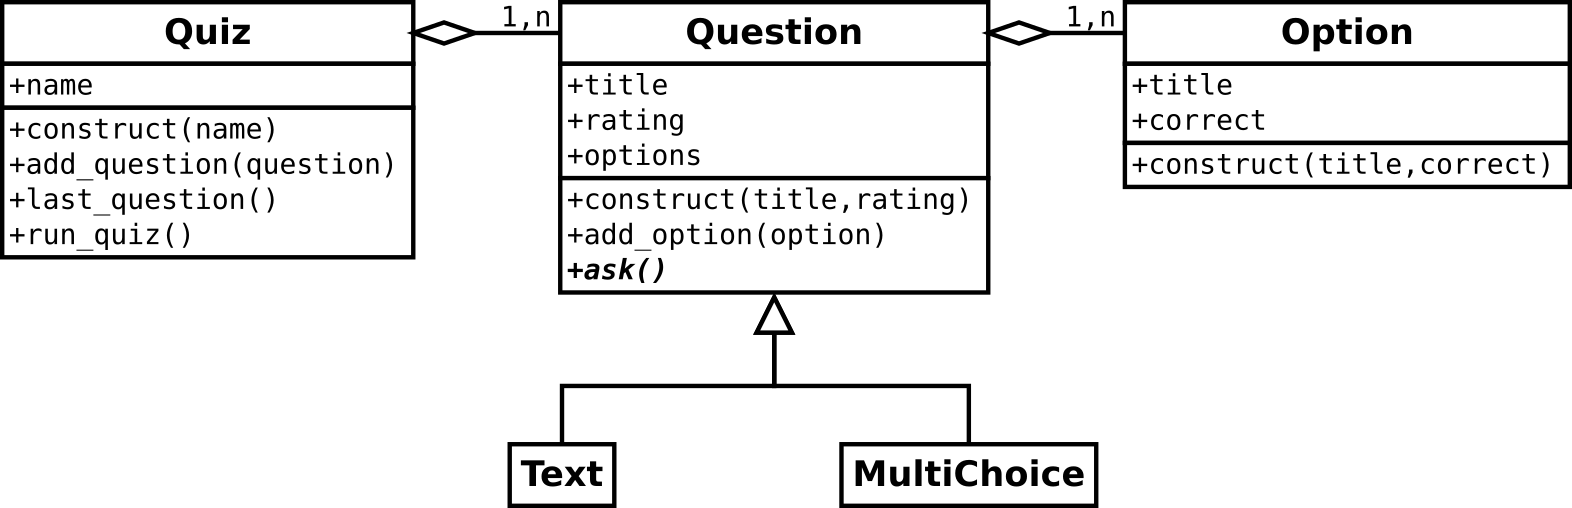
\includegraphics[scale=0.4]{test/sdl.png} 
\captionof{figure}{Diseño cuestionarios}
\end{center}
\hfill\\

Este programa ha sido modelado usando programación orientada a objetos. Se presenta un fichero de código fuente por cada clase que conforma el sistema de cuestionarios, otro fichero 
la definición del DSL junto con el flujo principal que conforma el motor de cuestionarios, y otro fichero que se corresponde con un cuestionario de ejemplo.\\

\begin{lstlisting}[language=omi]
#!/usr/local/bin/omi
#Sistema de cuestionarios
#=======================================================================
include "quiz.class.omi";
#=======================================================================
global quiz;
#=======================================================================
#Funciones del DSL 
~multichoice (text, rating) {
   quiz->add_question (new MultiChoice (text, rating));
}

~text (text, rating) {
   quiz->add_question (new Text (text, rating));
}

~option (text, correct = null) {
   quiz->last_question()->add_option(new Option (text, correct));
}
#=======================================================================
if (args[1]){
   title = args[2]?:"Sin titulo";
   << title;
   quiz =  new Quiz (title);
   include args[1];
   quiz->run_quiz();
}
else
   << "Debe indicar un cuestionario";
#=======================================================================
\end{lstlisting}
\captionof{lstlisting}{Cuestionarios: quiz.omi}
\hfill\\

\begin{lstlisting}[language=omi]
#quiz.class.omi
#=======================================================================
include "question.class.omi";
#=======================================================================
class Quiz {
   name = '';
   questions = {};
   ~ Quiz (name) {
      this->name = name;
   }
   ~ add_question (question) {
      this->questions[size this->questions] = question;
   }
   ~ last_question () {
      return this->questions [(size this->questions) - 1];
   }
   ~ run_quiz () {
      count = 0;
      total = 0;
      $(this->questions) {
         if ($->ask ()) count += $->rating;
         total += $->rating;
      }
      << "Tienes " << count << " respuestas correctas de " << total;
   }
}
#=======================================================================
\end{lstlisting}
\captionof{lstlisting}{Cuestionarios: quiz.class.omi}
\hfill\\

\begin{lstlisting}[language=omi]
#question.class.omi
#=======================================================================
include "option.class.omi";
#=======================================================================
class Question {
   title = "";
   rating = 0;
   options = {};
   ~ Question (title, rating) {
      this->title = title;
      this->rating = rating;
   }
   ~ add_option (option) {
      this->options [(size this->options)] = option;
   }
}
#-----------------------------------------------------------------------
class Text extends Question {
   ~ Text (title, rating) {
      this->Question (title, rating);
   }
   ~ ask () {
      << "";
      << this->title << " (" << this->rating << ")";
      << "Introducir respuesta: ";
      >> ans;
      n = size (this->options);
      for (i = 0; i < n; ++i) {
         if (ans == this->options[i]->title)
            return true;
      }
      return false;
   }
}
#-----------------------------------------------------------------------

class MultiChoice extends Question {
   ~ MultiChoice (title, rating) {
      this->Question (title, rating);
   }
   ~ ask () {
      << this->title << " (" << this->rating << ")";
      count = 0;
      $(this->options) <<  (++count) << " - " << $->title;
      << "Introducir respuesta: ";
      >> ans;
      return (this->options[ans - 1]) && this->options[ans - 1]->correct;
   }
}
#=======================================================================
\end{lstlisting}
\captionof{lstlisting}{Cuestionarios: question.class.omi}
\hfill\\

\begin{lstlisting}[language=omi]
#option.class.omi
#=======================================================================
class Option {
   title = "";
   correct = "";
   ~ Option (title, correct){
      this->title = title;
      this->correct = correct;
   }
}
#=======================================================================
\end{lstlisting}
\captionof{lstlisting}{Cuestionarios: option.class.omi}
\hfill\\

\begin{lstlisting}[language=omi]
#Ejemplo de cuestionario.
multichoice("Cuanto tiempo duro la guerra de los 100 a|{\color{red}\emph{ñ}}|os?", 2.5);
option (100, false);
option (116, true);
option (90, false);
option (102, false);
multichoice("Un s|{\color{red}\emph{í}}|mil es ...", 2.5);
option ("Una comparaci|{\color{red}\emph{ó}}|n", true);
option ("Una duda", false);
option ("Un aparato para medir el tiempo", false);
text ("En que provincia desemboca el rio Guadalquivir?", 2.5);
option("C|{\color{red}\emph{á}}|diz", true);
option("c|{\color{red}\emph{á}}|diz", true);
\end{lstlisting}
\captionof{lstlisting}{Cuestionarios: ejemplo}
\hfill\\

Para ejecutar el cuestionario en una terminal de comandos:\\

\begin{lstlisting}[language=bash]
prompt$ ./quiz_system.omi quiz.q "Cuestionario"
\end{lstlisting}
\captionof{lstlisting}{Cuestionarios: ejecución}
\hfill\\

\section{Tic-Tac-Toe}
\label{sec:tic-tac-toe}
El programa se divide en tres módulos, cada uno correspondiente a un fichero. En un fichero se disponen las funciones de entrada y salida, tales como
solicitar los datos de los jugadores, imprimir el tablero, etc. En otro fichero se encuentran las funciones de inteligencia artificial para el caso de 
jugadores de tipo máquina. Y en otro se encuentra el flujo principal correspondiente al bucle de juego.

\begin{lstlisting}[language=omi]
#IO.omi
#=======================================================================
~IOJugadores () {
   jugadores = {};
   for (i = 1; i <= 2; ++i) {
      << "Nombre Jugador " << i;
      >> nombre;
      << "Tipo Jugador " << i << " [ 0 => Humano, otro => Maquina ]";
      >> tipo;
      if (tipo != 0) 
         tipo = 1;
      jugadores [] = { 
         'nombre' : nombre,
         'tipo' : tipo,
         'token' : (( i == 1)?1:-1),
      };
   }
   return jugadores; 
}
#-----------------------------------------------------------------------
~ IOTablero (tablero) {
   for (i = 0; i < 3; ++i) 
      << IOToken(tablero[i][0]) << " or " 
         << IOToken(tablero[i][1]) << " or " 
         << IOToken(tablero[i][2]);
}
#-----------------------------------------------------------------------
~ IOToken (pos) {
   if (pos == 1) 
      return 'X';
   elif (pos == -1)
      return 'O';
   else
      return '#';
}
#-----------------------------------------------------------------------
~ IOMover (tablero) {
   do {
      << "Dame la fila";
      >> row;
      << "Dame la columna";
      >> col;
   }while (tablero[row][col] !== 0);
   return {row, col};
}
#-----------------------------------------------------------------------
~IOGanador (jugadores, ganador) {
   if (ganador == 1 ){
      << "El ganador es " << jugadores[0]["nombre"];
   }elif (ganador == -1){
      << "El ganador es " << jugadores[1]["nombre"];
   }else{
      << "La partida ha quedado en empate";
   }
}

#=======================================================================
\end{lstlisting}
\captionof{lstlisting}{Tic-Tac-Toe: IO.omi}
\hfill\\

\begin{lstlisting}[language=omi]
#AI.omi
#=======================================================================
~primerosMov (tablero) {
   if (!tablero[1][1]) 
      return {1,1};
   do {
      col = row = time () % 2;
      if (row == 1) row = 2;
      if (col == 1) col = 2;
   }while (tablero[row][col] !== 0);
   return {row, col};
}
#-----------------------------------------------------------------------
~ miniMax (A, turno){
	mejor = turno * -1; 
   minMov = 9; 
   poda = 1;
   Mov = 0;
   posicion = {0, 0};
	if (!(t_ganador = procesarTablero (A)) && !tableroLleno (A)){
		for (cont = 0; cont < 3 && poda; cont ++)
			for (cont2 = 0; cont2 < 3 && poda; cont2 ++){
				if ( A [cont] [cont2] == 0){
					A [cont] [cont2] = turno;
					actual = miniMax_R (A, turno * -1,0,Mov);
					if (turno == 1 ){
						if ( actual  >= mejor && Mov <= minMov){
							mejor =actual;
							posicion [0] = cont;
							posicion [1] = cont2;
							if (mejor == turno){
								minMov = Mov;
								if (mejor == 1 && minMov == 0)
									poda = 0;
							}
						}
					} else
						if ( actual <= mejor && Mov <= minMov){
							mejor =actual;
							posicion [0] = cont;
							posicion [1] = cont2;
							if (mejor == turno){
								minMov = Mov;
								if (mejor == 1 && minMov == 0)
									poda = 0;
							}
						}
					A [cont] [cont2] = 0;
				}
			}
	}
   return posicion;
}
#-----------------------------------------------------------------------
~ miniMax_R (&A, turno, nMov, &Mov){
	mejor = turno * -1;
   poda = 1; 
   minMov = 9 ;
	if (!(t_ganador = procesarTablero (A)) && !tableroLleno (A)){
		for (cont = 0; cont < 3 && poda; cont ++){
			for (cont2 = 0; cont2 < 3 && poda; cont2 ++){
				if ( A [cont] [cont2] == 0){
					A [cont] [cont2] = turno;
					actual = miniMax_R (A, turno * -1, nMov +1, Mov);
					if (turno == 1 ){
						if ( actual  >= mejor && Mov <= minMov){
							mejor =actual;
							if (mejor == turno){ 		
								minMov = Mov;
								if (mejor == 1 && minMov == 0)
									poda = 0;
							}
						}
					} else
						if ( actual <= mejor && Mov <= minMov){
								mejor =actual;
								if (mejor == turno){ 	
									minMov = Mov;
									if (mejor == 1 && minMov == 0)
										poda = 0;
							}
						}
					A [cont] [cont2] = 0;
				}
			}
		}
		Mov = minMov;
		return mejor;
	}
	Mov = nMov;
	return  t_ganador;
}
#-----------------------------------------------------------------------
~procesarTablero (A) {
   ganador = 0;
   cont = 0;
	for (cont = 0; cont < 3 && ganador == 0; cont ++){
		if (A [cont] [0] == A[cont] [1] && A [cont] [1] == A [cont] [2])
			ganador = A [cont] [1];
   }
	for (cont = 0; cont < 3 && ganador == 0; cont ++)
		if (A [0] [cont] == A [1] [cont] && A [1] [cont] == A [2] [cont])
			ganador = A [0] [cont];
	if (A [0][0] == A [1][1] && A [1][1] == A [2][2]  && ganador == 0 )
		ganador = A [0][0];
	if (A [0][2] == A [1][1] && A [1][1] == A [2][0] && ganador == 0)
		ganador = A [0][2];
	return ganador;
}
#-----------------------------------------------------------------------
~ tableroLleno (A){
	resp = 1;
	for (cont = 0; cont < 3 && resp; cont ++)
		for (cont2 = 0; cont2 < 3 && resp; cont2 ++)
			resp = A [cont] [cont2] != 0;
	return resp;
}
#=======================================================================
\end{lstlisting}
\captionof{lstlisting}{Tic-Tac-Toe: AI.omi}
\hfill\\

\begin{lstlisting}[language=omi]
#!/usr/local/bin/omi
#=======================================================================
include "IO.omi";
include "AI.omi";
#-----------------------------------------------------------------------
~juego () {
   tablero = {{0,0,0},{0,0,0},{0,0,0}};
   posicion = {0,0};
   turno = 0;
   jugadores = IOJugadores ();
   while (!(ganador = procesarTablero (tablero)) && !tableroLleno (tablero)){
      << "----------------------------------------------";
      IOTablero (tablero);
      << "\nTurno " << jugadores[turno%2]['nombre'];
      if (jugadores[turno%2]['tipo'] == 0) {
         posicion = IOMover (tablero);
      }else {
         << "Calculando movimiento...";
         if (turno <= 1) {
            posicion = primerosMov (tablero);
         }else {
            posicion = miniMax (tablero, jugadores[turno%2]['token']);
         }
      }
      tablero[posicion[0]][posicion[1]] = jugadores[turno%2]['token'];
      turno ++;
   }
   IOTablero (tablero);
   IOGanador (jugadores, ganador);
}
#-----------------------------------------------------------------------
juego ();
#======================================================================$
\end{lstlisting}
\captionof{lstlisting}{Tic-Tac-Toe: tic-tac.toe.omi}
\hfill\\

\section{Fibonacci}
\label{sec:fibonacci}
\begin{lstlisting}[language=omi]
#!/usr/local/bin/omi
#fibonacci.omi
#=======================================================================
~ fibonacci (n) {
   if (n == 1 || n == 2) 
      return 1;
   else 
      return fibonacci (n - 1) + fibonaci (n - 2); 
}
#-----------------------------------------------------------------------
<< fibonacci (args[1]);
#=======================================================================
\end{lstlisting}
\captionof{lstlisting}{Fibonacci}
\hfill\\

\section{N-body}
\label{sec:n-body}

\begin{lstlisting}[language=omi]
#!/usr/local/bin/omi
#=======================================================================
~ energy(&b) {
   e = 0.0;
   m = size (b);
   for (i=0; i < m; ++i) {
       b1=b[i]; 
       e += 0.5*b1[6]*(b1[3]*b1[3]+b1[4]*b1[4]+b1[5]*b1[5]);
       for (j=i+1; j<m; j++) {
         b2=b[j];
         dx=b1[0]-b2[0]; dy=b1[1]-b2[1]; dz=b1[2]-b2[2];
         e -= (b1[6]*b2[6])/sqrt(dx*dx + dy*dy + dz*dz);
       }
   }
   return e;
}

pi=3.141592653589793;
solar_mass=4*pi*pi;
days_per_year=365.24;

bodies = {
   {0.0, 0.0, 0.0, 0.0, 0.0, 0.0, solar_mass }, //Sun
   { 
      4.84143144246472090, //Jupiter
      -1.16032004402742839,
      -0.103622044471123109,
      0.00166007664274403694 * days_per_year,
      0.00769901118419740425 * days_per_year,
      -0.0000690460016972063023 * days_per_year,
      0.0009.54791938424326609 * solar_mass
   },
   {
      8.34336671824457987,    // Saturn
      4.12479856412430479,
      -0.403523417114321381,
      -0.00276742510726862411 * days_per_year,
      0.00499852801234917238 * days_per_year,
      0.00002.30417297573763929 * days_per_year,
      0.000285885980666130812 * solar_mass
   },
   {
      12.8943695621391310, // Uranus
      -15.1111514016986312,
      -0.223307578892655734,
      0.00296460137564761618 * days_per_year,
      0.00237847173959480950 * days_per_year,
      -0.0000296589568540237556 * days_per_year,
      0.0000436624404335156298 * solar_mass
   },
   {
      15.3796971148509165, // Neptune
      -25.9193146099879641,
      0.179258772950371181,
      0.00268067772490389322 * days_per_year,
      0.00162824170038242295 * days_per_year,
      -0.0000951592254519715870 * days_per_year,
      0.0000515138902046611451 * solar_mass
   }
};

// offset_momentum
px=py=pz=0.0;
for (bodies as e) {
    px+=e[3]*e[6]; 
    py+=e[4]*e[6]; 
    pz+=e[5]*e[6];
} 
bodies[0][3] = -1 * (px) / solar_mass;
bodies[0][4] = -1 * (py) / solar_mass;
bodies[0][5] = -1 * (pz) / solar_mass;

pairs = {};
m=size(bodies);
for (i=0; i<m; ++i) 
   for (j=i+1; j<m; j++) 
      pairs[] = {bodies[i], bodies[j]};

n = args[1];

<< energy(bodies);

i=0; 
do {
   for (pairs as p) {
      a=p[0]; b=p[1];
      dx=a[0]-b[0]; dy=a[1]-b[1]; dz=a[2]-b[2];

      dist = sqrt(dx*dx + dy*dy + dz*dz);
      mag = 0.01/(dist*dist*dist);
      mag_a = a[6]*mag; mag_b = b[6]*mag;
	
      a[3]-=dx*mag_b; a[4]-=dy*mag_b; a[5]-=dz*mag_b;
      b[3]+=dx*mag_a; b[4]+=dy*mag_a; b[5]+=dz*mag_a;
    } 

    for (bodies as b) {
        b[0]+=0.01*b[3]; b[1]+=0.01*b[4]; b[2]+=0.01*b[5];
    } 

} while(++i<n);

<< energy(bodies);
\end{lstlisting}
\captionof{lstlisting}{N-body}

